\chapter{Supplement to Chapter~\ref{art}}\label{app.art}
%===================================================================================================
\section{Objective~1}\label{app.art.1}
%---------------------------------------------------------------------------------------------------
\subsection{Scenario Cascades}\label{app.art.1.cascade}
Figure~\ref{fig:art.1.cascade} illustrates \dots % TODO
\begin{figure}[h]
  \centerline{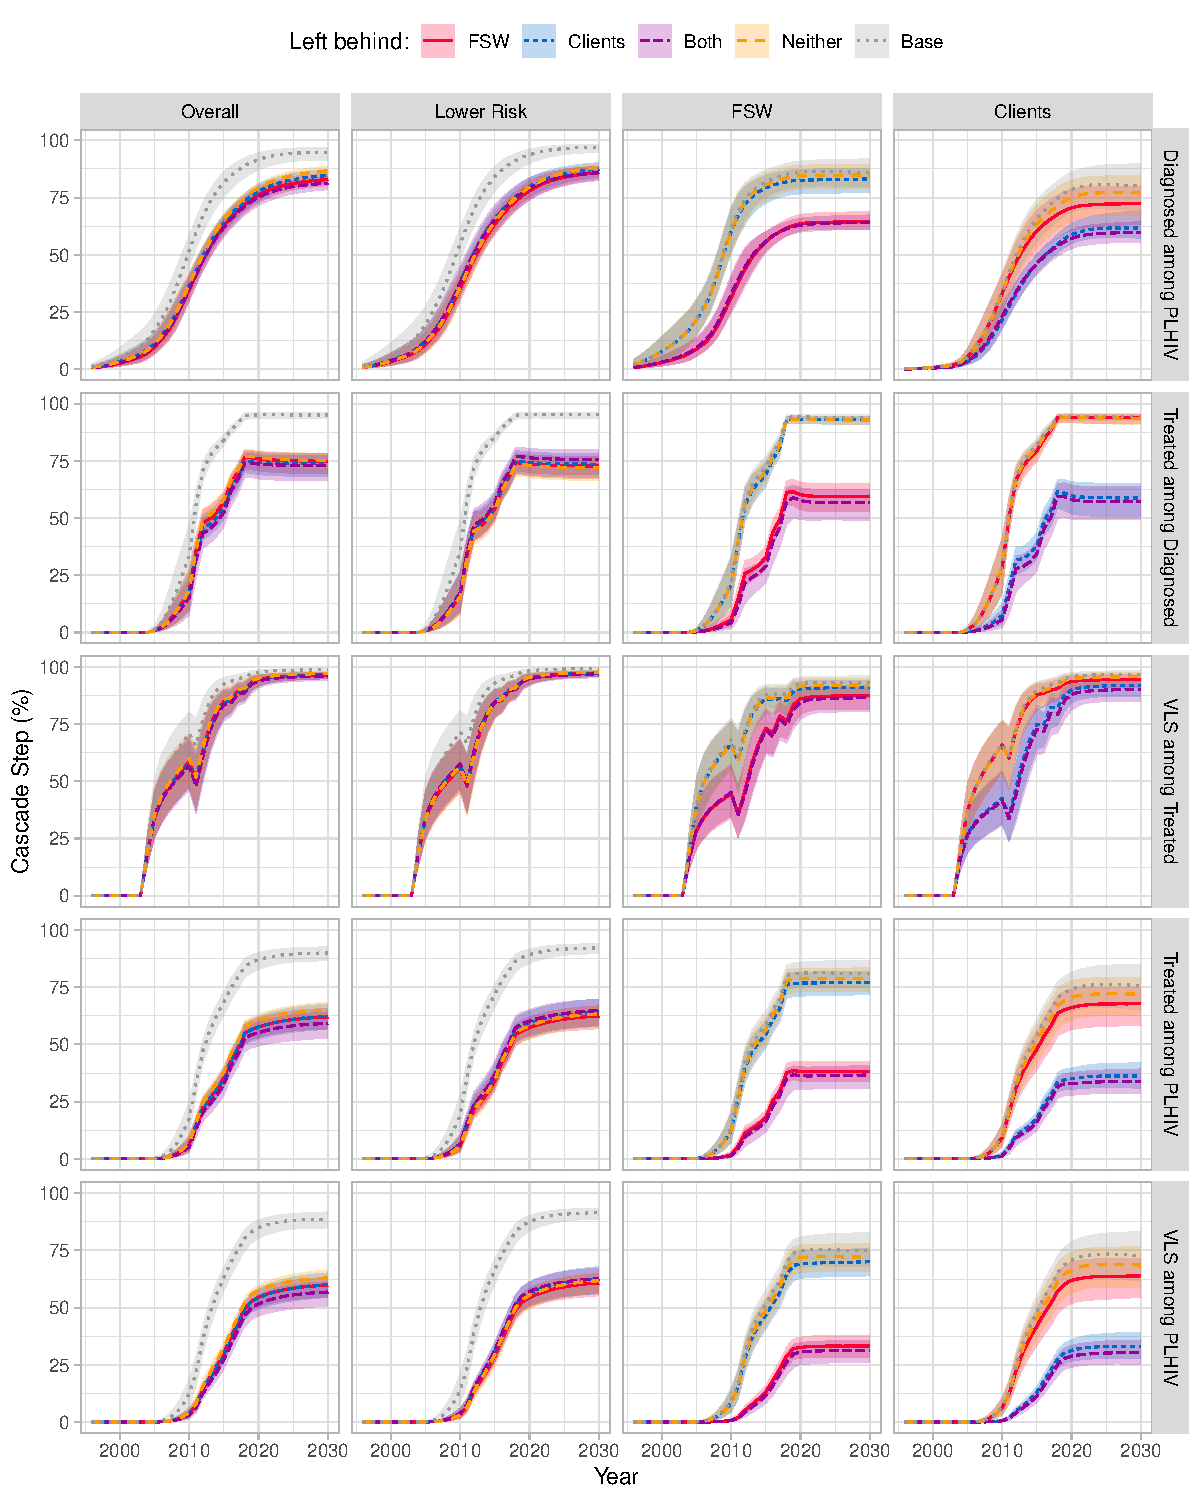
\includegraphics[scale=.8]{art.1.cascade}}
  \caption{Cascade attainment over time across scenarios}
  \label{fig:art.1.cascade}
  \floatfoot{\ffpopz; \ffart; \ffribbon.}
\end{figure}
%---------------------------------------------------------------------------------------------------
\subsection{Distributions of Additional Infections}\label{app.art.1.wiw}
As in \sref{model.res.wiw}, Figure~\ref{fig:art.1.wiw} illustrates \dots % TODO
\begin{figure}
  \subcaptionoverlap
  \foreach \var in {part,from,to}{
  \begin{subfigure}{\linewidth}
    \includegraphics[width=\linewidth]{art.1.wiw.\var}
    \caption{\raggedright}\label{fig:art.1.wiw.\var}
  \end{subfigure}}
  \caption{Additional infections in each ``who is left behind'' counterfactual scenario
    \vs the base case, stratified by:
    \sfref{fig:art.1.wiw.part} partnership type,
    \sfref{fig:art.1.wiw.from} transmitting group, and
    \sfref{fig:art.1.wiw.to} acquiring group}
  \label{fig:art.1.wiw}
  \floatfoot{\ffart; \ffwiw.}
\end{figure}
%===================================================================================================
\section{Objective~2}\label{app.art.2}
Figure~\ref{fig:art.2.cascade} illustrates \dots % TODO
\begin{figure}[h]
  \centering
  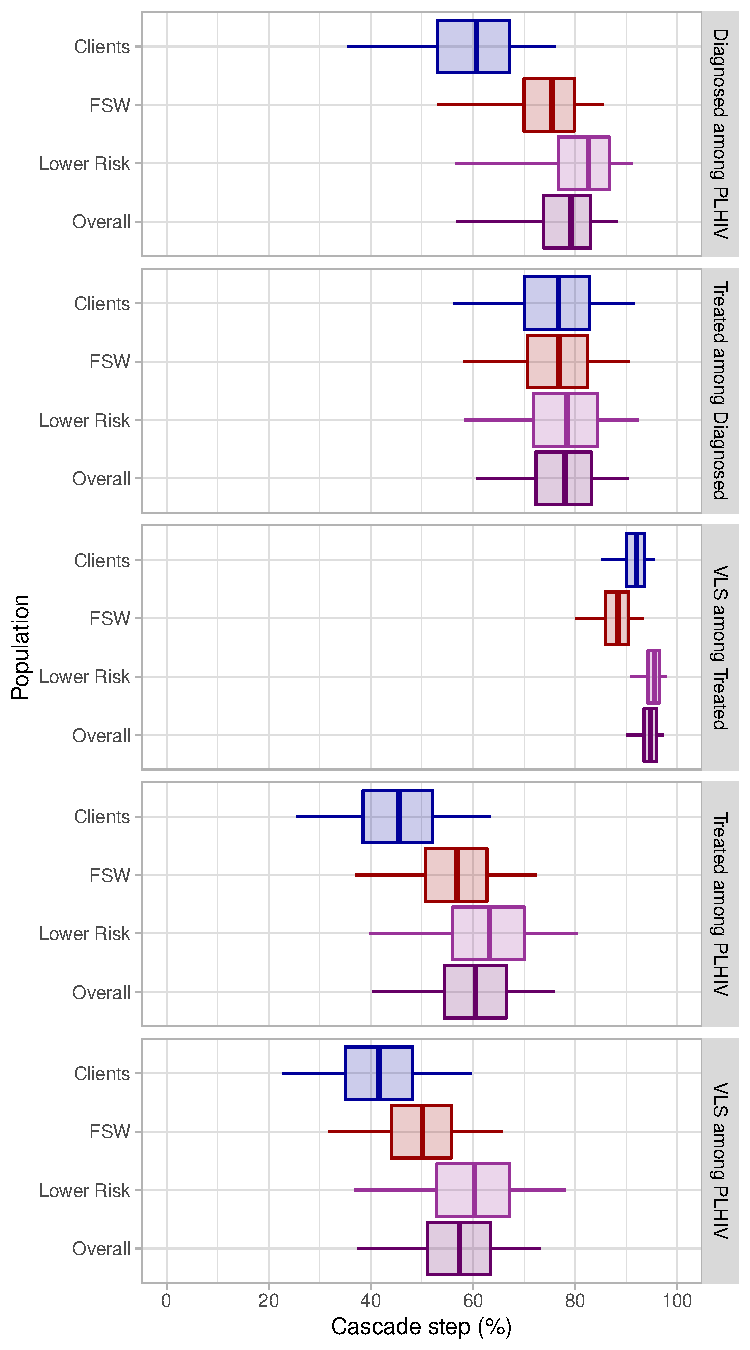
\includegraphics[scale=.8]{art.2.cascade}
  \caption{Cascade attainment by 2020 across samples}
  \label{fig:art.2.cascade}
  \floatfoot{\ffpopz; \ffbox.}
  % TODO: PLHIV, ffsens?
\end{figure}
